\documentclass[a4paper, 10pt, fleqn]{article}

\usepackage[utf8]{inputenc}
\usepackage[T1]{fontenc}
\usepackage{textcomp}
\usepackage{lmodern}
\usepackage[ngerman]{babel}
\usepackage{enumerate}

\usepackage{hyperref}
\usepackage{apacite}

\usepackage{color}
\usepackage{float}

\usepackage{amsmath}
\usepackage{graphicx}

\usepackage{listings}
\lstset{language=[ansi]C++}

\title{Termpaper - KeyEscrow}
\author{Daniel Foehn, Silvio Stappung, Jonas Hansen}
\date{\today} %Es kann ein bestimmtes Datum eingetragen werden

\graphicspath{{images/}}

%macro definitions
\definecolor{shadecolor}{RGB}{200,200,200}
%small colored box with no visible border, breaks before and after box
\newcommand{\shadebox}[1]{\par\noindent\colorbox{shadecolor}
{\parbox{\dimexpr\textwidth-2\fboxsep\relax}{#1}}}
%small noncolored box with visible border, breaks before and after box
\newcommand{\commandbox}[1]{\par\noindent\fbox{\begin{minipage}{\textwidth}#1\end{minipage}}\par\noindent}

\begin{document}
\maketitle
\tableofcontents
\listoffigures
\listoftables
\clearpage
\section{Abstract}

\clearpage
\section{Einleitung}
Die Verschlüsselung von Daten hat in den vergangenen Jahren drastisch an Bedeutung gewonnen. 

 % Aufkommen der Verschlüssenung --> von symetrisch zu asymetrisch 
 % Geheimdienste vor Herausforderung (Interessenskonflikt <-> Sicherheit, Datenschutz)
 % Sensibillisierung der Enduser (kein Neuland)
 % Problematiken
 % KEY ESCROW!!!!!!!!!!

\clearpage
\section{Aktuelle Situation}
	
Das folgende Kapitel bietet einen Einblick in die rechtliche und geschichtliche Situation zur Hinterlegung von Schlüsseln, sowie einen Abriss über die allgemeine sicherheitspolitische Lage im Hinblick auf die Kryptografie von elektronischen Daten.
	
	
	\subsection{Situation der Schweiz}
		% Silvio

Die sicherheitspolitische Lage wurde auch in der Schweiz in den vergangenen Jahren nicht einfacher. Trotzdem ist auch in der Schweiz das Hinterlegen von kryptographischen Schlüsseln kein neues Thema. \\
Wie in anderen Ländern ist auch in der Schweiz das Hauptargument für staatlichen Zugang zu kryptografischen Schlüsseln die Bekämpfung des Terrorismus. Auch bereits im Jahr 2005 wurde von der sicherheitspolitischen Kommission des Nationalrates ein Postulat eingereicht, welches unter anderem auch die Dechiffrierung von Kommunikationsverbindungen vereinfachen vorsah. \cite{adminch} \\ % (KP 7.1. / 7.2.)
Zu diesem Zeitpunkt wurde von staatlicher Seite her vor Allem an der Dechiffrierung von Daten gearbeitet, welche hauptsächlich im Bereich der militärischen Funkaufklärung zu gunsten des strategischen Nachrichtendienstes durchgefüphrt wurde. Da mit der Zeit die Verschlüsselungsalorithmen und auch deren Schlüssel immer stärker und schwerer zu brechen waren, wurde unter anderem Vorgeschlagen, ein Key Escrow System zur Hinterlegung aller kryptografischen Schlüssel zu erstellen und die Verwendung von nicht hinterlegten Schlüsseln unter Strafe zu stellen. Als etwas weniger strenge alternative wurde auch die Hinterlegung der Algorithmen, anstelle der Schlüssel, diskutiert, da dies technisch im Vergleich einfacher umzusetzen wäre. \cite{adminch} \\ 
\\ %(KP 7.2.)
Die Einführung eines Key Escrow Systemes für die Schweiz wurde schlussendlich vom Bundesrat aufgrund der folgenden Punkte abgelehnt \cite{adminch}: % KP 7.3

\begin{itemize}
  \item bereits eingeführte kryptografische Systeme müssten ersetzt werden
  \item Politisch nicht durchsetzbar aufgrund der hohen Einführungskosten
  \item zentraler Keystore wäre ein Riskantes Ziel für Cyberangriffe
  \item massive Kosten für Administration und Unterhalt des Systems
\end{itemize}

Zudem würde man auch nach erfolgreicher Einführung eines Key Escrow Systemes vor einigen Problemen stehen. Verstösse gegen das Verschlüsselungsverbot mit nicht hinterleten Schlüsseln wäre hierbei kaum Nachweisbar und somit von Staatlicherseite nicht verfolgbar. \cite{adminch} \\%KP 7.3.
\\
Auch das neue Nachrichtendienstgesetz, welches voraussichtlich im Jahr 2017 in Kraft treten soll, befasst sich stark mit der Informationsbeschaffung und somit auch mit der Entschlüsselung von Daten. Trotzdem ist  zehn Jahre nach der oben erwähnten Debatte von Key Escrow keine Rede mehr. \cite{ndgesetz} \cite{botschaftndg} \\ %Nachrichtendienstgesetz 1 & 2
		
	\subsection{Situation im Aussland}
		% Silvio
		
Auch im Aussland ist Key Escrow ein altbekanntes Thema. Bereits Anfangs der Neunzigerjahre wurde in den USA unter Präsident Clinton mehrmals über die Einführung eines solchen Systemes beraten. \cite{adminch} \cite{denning} %Kp 7.3. Bericht Bund / Gregg Bericht
Desshalb ist es auch nicht verwunderlich, dass nach den Anschlägen vom 11. September 2001 von diversen amerikanischen Politikern ein Key Escrow System gefordert wurde. \\
Der wohl einflussreichste Politiker, welche selbige Forderung stellte war der republikanische Senator Judd Gregg, welcher am 13. September 2001 ein neues Regime im Hinblick auf die Verschlüsselung forderte. Judd Gregg forderte dabei die zentralisierte Speicherung aller Schlüssel für in Amerika gebauten sowie importierten kryptografischen Produkte. Die Regierung Bush's hat dieses Begehren allerdings abgelehnt und auch keine weiteren Massnahmen in der Verschlüsselungspolitik zur Terrorbekämpfung vorgeschlagen. \cite{denning}\\ %Gregg Bericht
\\
Doch auch in der heutigen Zeit gibt es immer wieder Forderungen nach staatlichem Einsicht in alle verschlüsselten Verbindungen. Analog wie früher geschieht dies wieder unter dem Deckmantel der Terrorbekämpfung und auch in Europa. Ein Beispiel dafür ist der britische Premierminister David Cameron, der sich, im Hintergrund der Anschläge auf das Satieremagazin "Charlie Hebdo" in Paris von Anfangs Januar 2015, zu diesem Thema äusserte. \\
Cameron forderte ein allgemeines Verbot von jeglicher Kommunikation, welche von staatlicher Seite her nicht mitgelesen werden kann. Allerdings wird diese Forderung von vielen Stellen als starken Angriff auf die Privatsphäre erachtet. \cite{insideit} \\%Cameron
Auf der anderen Seite zeigte der Fall "Edward Snowden" auch die Praktiken des Amerikanischen Geheimdienstes NSA sowie dessen britischen Pendant GCHQ auf, wie diese Staatlichen Organisationen jegliche Art von Informationen zu entschlüsseln versuchen. Auch der Chef der NSA, Michael Rogers, forderte die Hinterlegung von kryptografischen Schlüsseln zur Entschlüsselung zuhanden der Geheimdienste. Dabei verfolgte er einen etwas anderen Ansatz. Rogers schlug vor, die Schlüssel verteilt bei verschiedenen Stellen zu hinterlegen, welche nur zusammen den eigendlichen Schlüssel generieren können. Dies ist ein bekannter Ansatz, wie er bei vielen grösseren sicherheitsrelevanten Einrichtungen verwendet wird. \\
Diese Escrow Pflicht würde sich allerdings nur auf US-Hersteller auswirken und hätte keinen Einfluss auf ausländische Unternehmungen. \cite{annabiselli} \\ % Netzpolitik
\\
Auch im Aussland lässt sich sagen, dass im allgemeinen viel über das Thema der staatlichen Einsicht in verschlüsselte Daten diskutiert wird. Allerdings sehen die meissten Staaten aufgrund des Aufwandes, der Kosten sowie der sicherheitstechnischen Bedenken von Key Escrow Systemen ab und wenden nich der herkömmlichen Entschlüsselung der Daten zu.


		
	\subsection{Position von Experten}
		% Dani

\clearpage
\section{Anwendungsgebiet}
	Das folgende Kapitel zeigt mögliche Anwendungen von Key Escrow Systemen und deren Alternativen für den Gebrauch von staatlichen Behördern, sowie in der Privatwirtschaft auf.
	
	\subsection{Staatlich}
		% Silvio
Die immer stärker werdenden kryptografischen Verfahren stellen die staatlichen Sicherheitsbehördern vor immer grössere Probleme. Die Anwendung von Verschlüsselung durch Straftäter erschwert die Arbeit der Sicherheutsbehörder enorm. \\
Nach terroristischen Anschlägen werden immer wieder Stimmen laut, welche die Einführung einer Möglichkeit zur Erleichterung der Entschlüsselung von Kommunikationsdaten fordern \cite{insideit} \cite{annabiselli} \cite{denning}. 
Dabei werden immer wieder die selbigen Themen angesprochen:

	\subsubsection{Erstellung eines Key Escrow Systemes}
Die Einführung eines Key Escrow Systemes wäre für jeden Geheimdienst wohl das höchste aller Gefühle. Allerdings hat ein staatliches Key Escrow System politisch einen sehr schweren Standpunkt. Dies liegt vor allem daran, dass ein solches System zu einem gewaltigen Verlust, wenn nicht gerade eine totale Aufgabe der Privatsphäre zur Folge hätte und die Gesellschaft kaum mit einer so drastischen Massnahme einverstanden wäre.\cite {insideit} \\
Fraglich wäre auch der Nutzen des Sytems im Hinsicht auf grössere kriminelle Organisationen. Zu glauben, dass alle Kriminellen Verschlüsselungstools benutzen würden, für welche der Schlüssel im Escrow System hinterlegt ist wäre sehr fraglich. Beispielsweise hat die Terrororganisation Al-Qaida von der Organisation nahestehenden Kryptologen ein eigenes Verschlüsselungssystem entwickeln lassen \cite{denning}. Dass es sich dabei nicht im einen Einzelfall handelt, lasst sich auch stark annehmen.
	
	\subsubsection{Hinterlegung von verwendeten Verschlüsselungsalgorithmen}
Eine nicht so schwerwiegende Alternative zu Key Escrow wäre die Hinterlegung des Verschlüsselungsverfahrens ohne Hinterlegung des verwendeten kryptografischen Schlüssels. Diese Hinterlegung sollte zum Nutzen haben, dass den Strafverfolgungsbehörden die Arbeit etwas erleichtert würde. Dies hätte allerdings auch nur dann einen Nutzen, wenn nur schwächere oder Algorithmen mit einer Sicherheitslücke verwendet werden dürfen. Diese Lücken wären somit auch ein Eigentor für die Sicherheitsbehörden, da sie somit Kriminellen eine weiter Angriffsfläche auf die Bürger bieten würden. \cite{adminch} % KP. 7.3.

	
	\subsubsection{Verbot von alternativen Verschlüsselung}
Mit der Einführung eines Escrow Systemes oder der Einführung einer Hinterlegungspflicht für Algorithmen würde auch dazu führen, dass die Gegenseite, das heisst die Verwendung nicht hinterlegter Schlüssel / Algorithmen, verboten werden müsste. Auf der einen Seite wäre ein solches Verbot sehr schwer durchzusetzten, geschweige überhaupt zu kontrollieren, auf der andern Seite wäre es von der Strafnorm her auch kaum möglich, eine genug hohe Maximalstrafe ansetzen zu können, um grössere kriminelle Organisationen von der illealgen Verwendung der Verschlüsselung abzuwenden. \cite{adminch} \\ %KP 7.3.
Zudem wäre ein solches Verbot auch nur dann vernünftig brauchbar und durchsetzbar, wenn es von der internationalen Gemeinschaft getragen und somit in allen Ländern durchgesetzt würde \cite{denning}. Da der Internationale Weg in Sache Verschlüsselungspolitik in eine andere Richtung weht, zeigt sich darin, dass sich einige Länder, welche in den neunziger Jahren die Kryptografie noch eingeschränkt hatten, in Richtung einer offenen Kryptografiepolitik bewegen. \cite{clipperchip} \cite{adminch} \\ % 7.2.3
Eine Einführung eines solchen Verbotes würde einen Staat Interational stark ins Abseits setzten und das Verbot wäre somit auch kaum duchsetzbar.
		
	\subsection{Firmenintern}
Das nachfolgende Kapitel gibt einen Überblick über die Problembereiche beim Key Management von Firmen und zeigt auf, inwiefern Hintertüren für staatliche Eingriffe in Software eingebaut werden können.

	\subsubsection{Key Management Systeme (KMS)}
Das zentrale Verwalten und hinterlegen von Schlüsseln ist für grössere Firmen eine Notwendigkeit. \\
Geschäftskritische Daten sollten wenn immer verschlüsselt werden. Um den Überblick über die verwendeten Schlüssel zu bewahren, werden Key Management Systeme (KMS) eingesetzt.
Mit diesen Systemen lassen sich folgende Problembereiche addressieren:
\begin{itemize}
	\item Datensicherheit durch Verschlüsselung gewährleisten
	\item Zentrales Verwalten und Administrieren von Schlüsseln
	\item Entschlüsseln von Geschäftsdaten von Mitarbeitenden bei Tod oder Abwesenheit
	\item Entschlüsseln von Geschäftsdaten bei untreuen Mitarbeitern
  \item Überwachung von Mitarbeitern
  \item Verwalten und verteilen von Softwarelizenzen
\end{itemize}
	

	\subsection{Clipper Chip / Escrowed Encription Standard (EES)}
\begin{figure}[H]
	\centering
	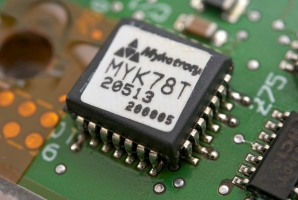
\includegraphics[width=.8\textwidth]{clipper-chip.jpg}
	\caption{MYK-78 Clipper Chip (1993)}
	\label{fig:clipper-chip}
\end{figure}
Ein exemplarisches Beispiel für staatliches erzwungenes Key Escrow ist der sogenannte Clipper Chip, welcher im Jahre 1993 durch die US-Behörden vorgestellt wurde und von der NSA entwickelt wurde.\\
Der Clipper Chip gehört zum Escrowed Encryption Standard (EES), welche hardwaremässige Verschlüsselung mit einer staatlich eingebauten Hintertür bietet. Die Behörden konnten die Verschlüsselungsmechanismen für jeden Clipper Chip rückgängig machen und so an die ursprünglichen Daten kommen. \\
Eingesetzt werden sollte der Chip staatlicher und privater Kommunikation. Der Haupteinsatzzweck lag bei verschlüsselter Telefonie. \cite{ees}\\
Entworfen wurde der Chip von Mykrotronx, hergestellt von VLSI Technology Inc. \\

	\subsubsection{Funktionsweise und Aufbau}
Der Clipper Chip verwendet zur Verschlüsselung den Skipjack-Verschlüsselungsalgorithmus welcher dem DES-Algorithmus ähnelt. Entwickelt wurde Skipjack von der NSA und wurde bis zur Veröffentlichung im Jahre 1998 unter Verschluss gehalten. Nur wenige zivile Experten erhielten Einsicht in den Sourcecode. \cite{ees}\\
Zentrales Element der nach EES verschlüsselten Kommunikation ist das \textit{Law Enforcement Access Field (LEAF)} welches bei der Kommunikation zwischen zwei Geräten mitgeschickt wird.\\
Der Aufbau des 128bit grossen LEAF sieht wie folg aus:
\begin{itemize}
	\item \textbf{Unit ID} (32 bit): Eindeutige ID pro Chip (bei Herstellung vergeben)
	\item \textbf{Encrypted Session Key} (80 bit): Session Key, verschlüsselt durch gerätespezifischen Unit Key
	\item \textbf{Checksum} (16 bit): Zur Fehlerüberprüfung
\end{itemize}
Wünschen zwei EES-fähige Geräte eine verschlüsselte Kommunikation, handeln diese als erstes einen eindeutigen, temporären \textit{Session Key} aus. Dieser wird mittels eindeutigem, gerätespezifischen Unit Key verschlüsselt. Das somit generierte LEAF wird zusätzlich mit einem \textit{Family Key} verschlüsselt, welcher pro EES-Gerätefamilie eindeutig ist.\\
Nachfolgend werden die verwendeten Keys zusammengefasst:
\begin{itemize}
	\item \textbf{Unit Key}: Eindeutig pro Clipper Chip.
	\item \textbf{Session Key}: Temporärer Key für eine Session. Wird bei Kommunikationsbeginn von den beiden Geräten ausgehandelt. 
	\item \textbf{Family Key}: Eindeutig pro EES-Gerätefamilie
\end{itemize}
\begin{figure}[H]
	\centering
	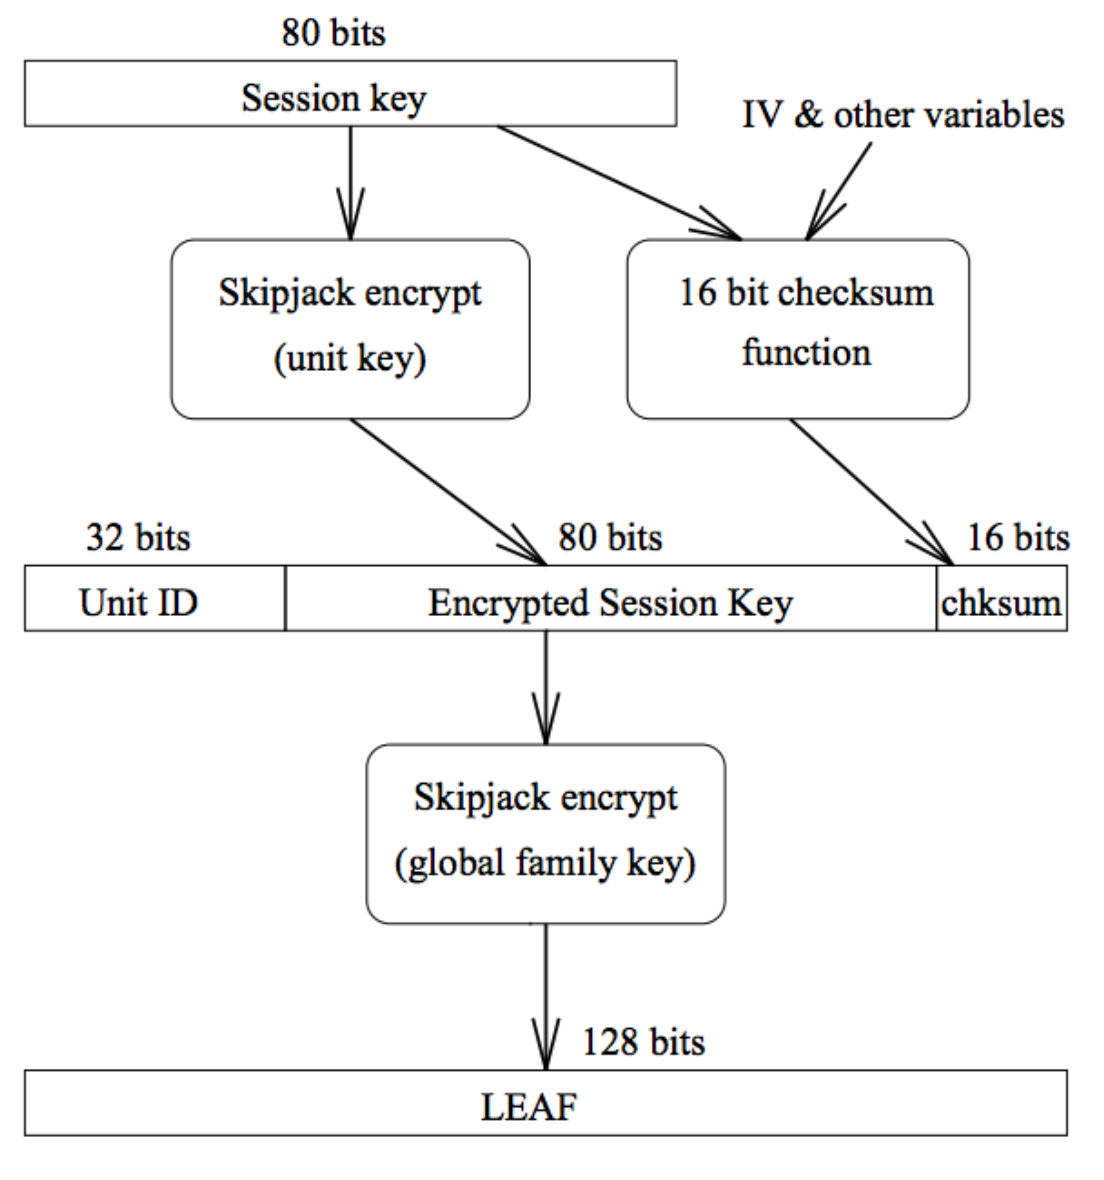
\includegraphics[width=.8\textwidth]
		{leaf-aufbau.png}
	\caption{Aufbau LEAF gemäss}
	{\cite{ees}}
	\label{fig:leaf-aufbau }
\end{figure}
Der \textit{Unit Key} wird dabei aufgespalten und bei zwei voneinander getrennten nationalen Behörden gespeichert. Dies dient dazu, Amtsmissbrauch einzudämmen. Soll aufgrund einer richterlichen Anordnung eine verschlüsselte Kommunikation abgehört werden, wird das LEAF mittels \textit{Family Key} dechiffriert. Daraus kann die Unit ID gewonnen werden. Mit der ID wird bei den beiden Behörden die beiden Teile des \textit{Unit Key} angefordert und zusammengefügt. Daraus kann danach der \textit{Session Key} und aus diesem wiederum die verschlüsselten Daten entschlüsselt werden.
\begin{figure}[H]
	\centering
	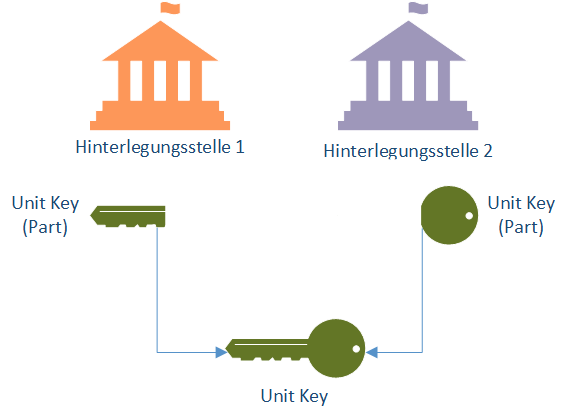
\includegraphics[width=.8\textwidth]
		{EES-Hinterlegungsstelle.png}
	\caption{Der Unit Key wird für den Schutz vor Amtsmissbrauch gesplittet an zwei Stellen hinterlegt. Beide Teile fügen sich zum gesamten Key zusammen.}
	{\cite{ees}}
	\label{fig:leaf-aufbau }
\end{figure}\\
Die Idee Clipper Chips kam bei der Bevölkerung überhaupt nicht gut an. \textit{"You don't want to buy a set of car keys from a guy who specializes in stealing cars"}, kommentierte Marc Rotenberg vom Electronic Privacy Information Center die Pläne der Behörden. \cite{ees_nytimes}\\
Bis im Jahre 1996 wurde der Clipper Chip irrelevant und wird seither nicht mehr weiter produziert. Parallel zum Clipper Chip wurden starke, frei verfügbare Datenverschlüsselungsmechanismen wie etwa PGP (Pretty Good Privacy) auf den Markt gebracht, welche die Idee eines staatlich kontrollierten Escrow-Systems verdrängten. Die Bevölkerung und Hersteller traute den Behörden zu wenig.

	\subsection{Recovery Agents und Trusted Third Parties}
Bei Key Escrow handelt es sich um ein Verfahren um Schlüssel für den späteren Gebrauch zu hinterlegen. Key Recovery ist der Prozess der Schlüssel anhand bestehender Daten rekonstruiert.
\\
Falls Key Recovery, beziehungsweise Key Escrow von zwei Parteien erwünscht ist, wird meist eine Trusted Third Party als unabhängige Kontroll- und Aufsichtsinstanz hinzugezogen.
\\
Die ausführende Instanz für Key Escrow und Key Recovery ist als Teil einer Trusted Thir Party der Recovery Agent.
		\subsubsection{Recovery Agent als Man in the Middle bei symmetrisch verschlüsselter Kommunikation}
Die beiden nachfolgenden Abbildungen illustrieren eine einfache funktionsweise eines Recovery Agent gemäss Belser \cite{isss}.
\begin{figure}[H]
	\centering
	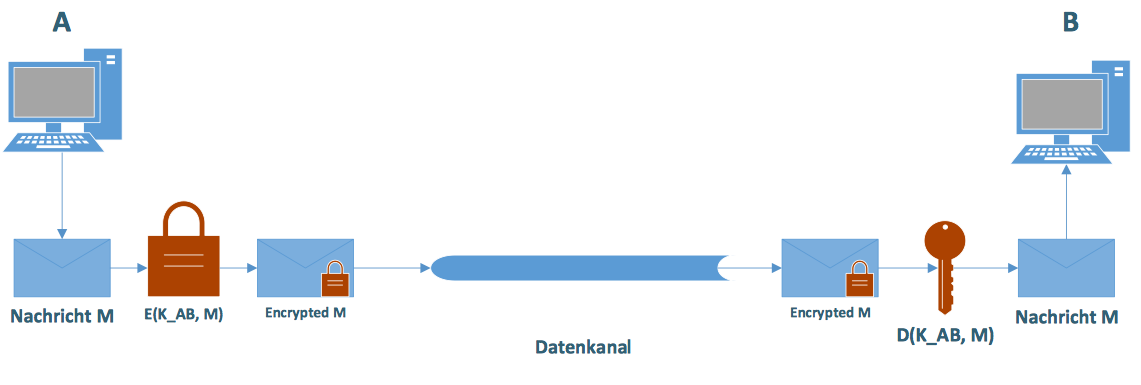
\includegraphics[width=.8\textwidth]
		{recovery-agent-aufbau.png}
	\caption{Symmetrische Verschlüsselung einer Kommunikation}
	\label{fig:recovery-agent-aufbau}
\end{figure}
In Abbildung \ref{fig:recovery-agent-aufbau} werden zwei kommunizierende Computer dargestellt. \textit{A} nimmt die Rolle des Senders und \textit{B} die Rolle des Empfängers ein. Sie nutzen zur Verschlüsselung der Nachricht ein symmetrisches Chiffrierverfahren. Der genutzte Schlüssel $K_{AB}$ wurde bereits ausgetauscht. \textit{A} erstellt die Nachricht $M$ und chiffriert sie mittels $E(K_{AB},M)=M_{C}$. Die chriffrierte Nachricht $M_{C}$ wird über den Datenkanal übertragen und von \textit{B} empfangen. Nach Dechiffrierung mittels $D(K_{AB},M_{C})=M$ kann die Nachricht $M$ von \textit{B} weiterverarbeitet werden.
\begin{figure}[H]
	\centering
	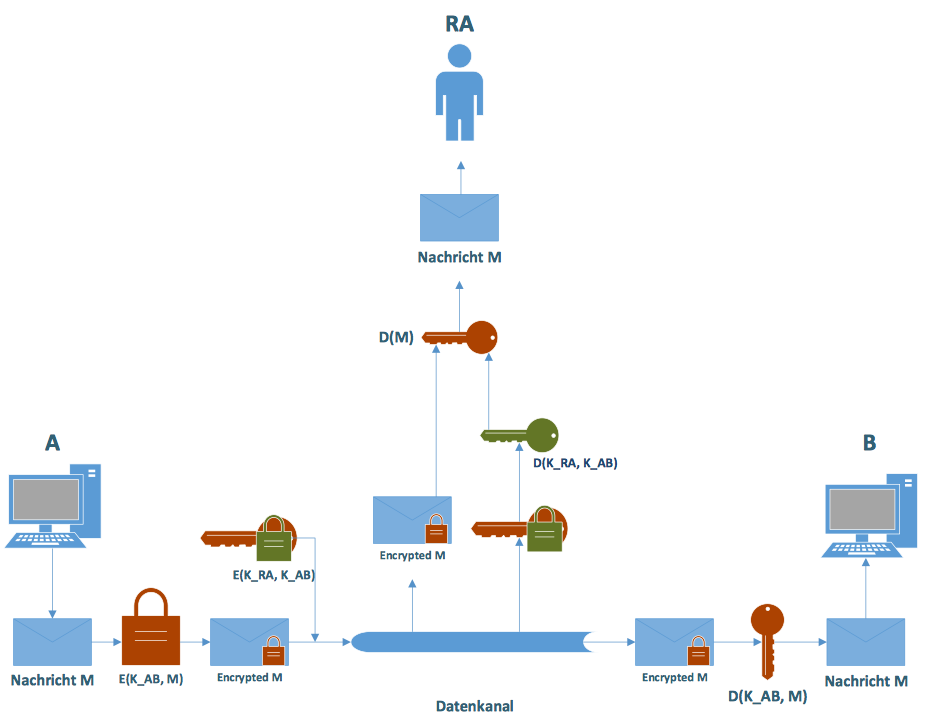
\includegraphics[width=.8\textwidth]
		{recovery-agent-mitm.png}
	\caption{Recovery Agent als Man in the Middle}
	\label{fig:recovery-agent-mitm}
\end{figure}
Abbildung \ref{fig:recovery-agent-mitm} erweitert die symmetrisch verschlüsselte Kommunikation von \textit{A} und \textit{B} mit einem Recovery Agenten \textit{RA}.
\\
Dieser besitzt ebenfalls einen Schlüssel $K_{RA}$. Beim Senden der Nachricht $M$ wird ebenfalls der chiffrierte Schlüssel $E(K_{RA},K_{AB})=C_{K_{AB}}$ von \textit{A} übertragen. Der Recovery Agent \textit{RA} hört die chiffrierte Nachricht $M_{C}$ und den chiffrierten Schlüssel $C_{K_{AB}}$ vom Datenkanal ab. Er dechiffriert den Schlüssel von \textit{A} und \textit{B} mittels $D(K_{RA}, C_{K_{AB}})=K_{AB}$ und kann somit auch die chiffrierte Nachricht $M_{C}$ dechiffrieren.


\clearpage
\section{Praktisches Beispiel}
	 	\subsection{Abhören von verschlüsselter Kommuniktion bei bekannten Schlüsseln}
	% TODO@16.11.
	\begin{figure}[H]
		\centering
		%\includegraphics[width=.8\textwidth]{""}
		\caption{Darstellung Versuchsaufbau}
		\label{fig:versuchsaufbau}
	\end{figure}
	\commandbox{conf t}
	\commandbox{monitor session 1 source interface Fa0/1}
	\commandbox{monitor session 1 destination interface Fa0/21 encapsulation repliate}
	\subsection{Analyse von bereits vorhandenen Tools} % keine Enterprise-lösungen

\clearpage
\section{Zukunftsaussichten}

\clearpage
\section{Fazit}

%to include all source in the literature index
\nocite{*}
\clearpage
\bibliography{bibliography}
\bibliographystyle{apacite}

\end{document}
